%%
%% Template chap2.tex
%%

\chapter{Implementing Fingerprint Indexing}
\label{cha:method}

\section{Structure of \beagle}
\label{sec:initial}

To be able to make any significant contribution to the \beagle\ project, I first
had to gain a solid understanding of the existing Scala codebase.

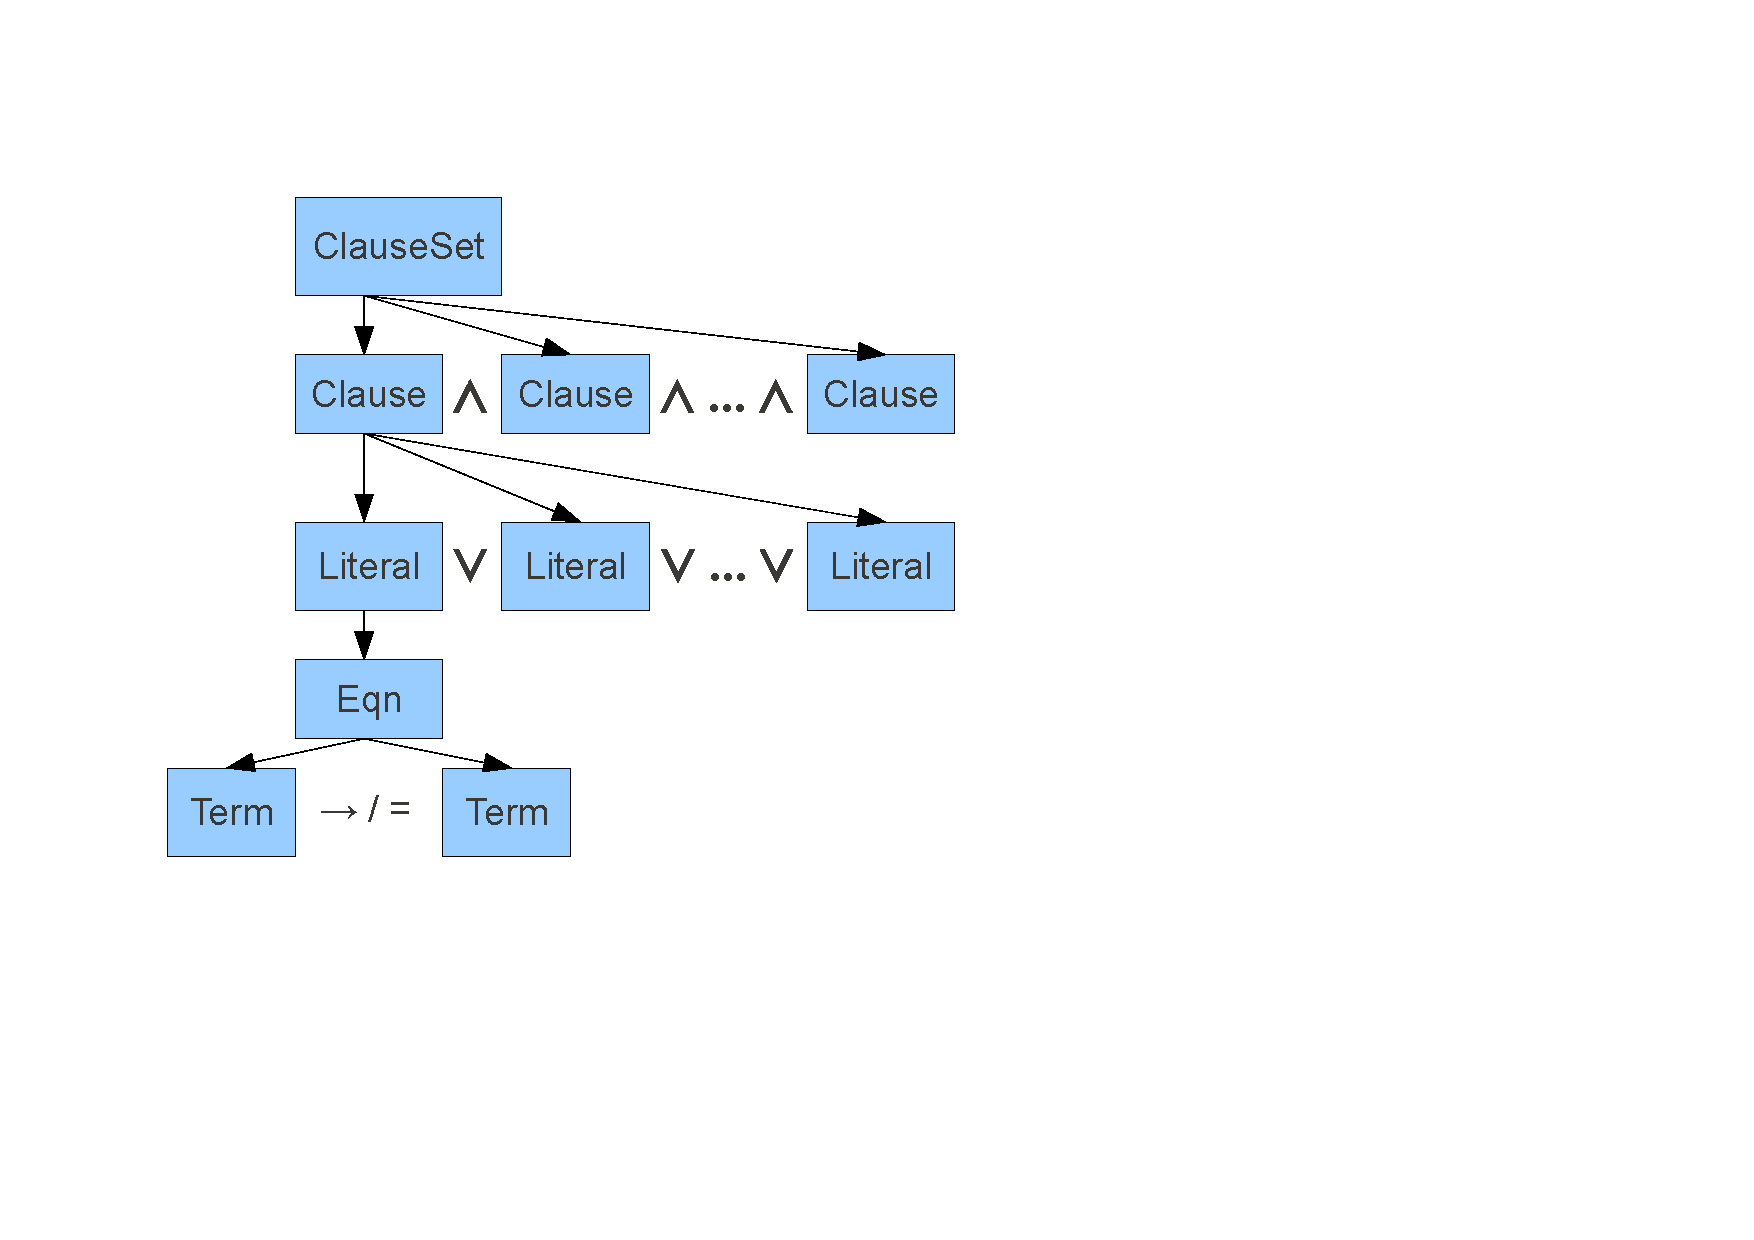
\includegraphics[clip,trim=2.5cm 5cm 10cm 2cm,width=\textwidth]{resources/logicstructure}

Describe main inference loop

Refer to results for instrumentation; showing what may be improved with indexing.

\section{Implementing Fingerprint Indexing}
\label{sec:initial}

The first step in adding Fingerprint Indexing to \beagle\ is creating the indexer
itself; a Scala class which will manage the index and provide functions for adding
to/retreiving from the Index. 

\subsection{Adding terms to the index}


The following block of Scala code extracts a single Fingerprint Feature from
a Term at the given position.
\begin{listing}[H]
\begin{scalacode}
 /** Extract the operator at position pos. Note that matching Var
   * and Funterm is an exhaustive pattern for Term. */
  def extractFeature(term: Term, pos: Position) : FPFeature = pos match {
    case Nil     => term match {
      case t:FunTerm => FPF(t.op) // Found function symbol, return it
      case t:Var     => FPA       // Found variable, return A
    }
    case p :: ps => term match {
      case t:FunTerm => try   {extractFeature(t.args(p), ps) }
                        //Attempted to index non-existent position, return N
                        catch {case e:IndexOutOfBoundsException => FPN}
      // Found variable BEFORE end of position, return B
      case t:Var     => FPB 
    }
  }
\end{scalacode}
\caption{Scala code to extract fingerprint features for matching.}
\label{lst:posextract}
\end{listing}

\subsection{Retrieving Compatible terms}

To compare two fingerprints with each other we look at them side-by-side and check
that each position shows a Y in the Fingerprint unifcation table. 
\begin{listing}[H]
\begin{scalacode}
 /** Check two Fingerprint features for compatibility based
   * on the unification table (See page 6 of [Shulz 2012]).
   * This table is reduced to 4 cases:
   *  - True if Features are equal,
   *  - True if at least one Feature is B,
   *  - True if at least one Feature is A; but no Ns,
   *  - False otherwise  */
  def compareFeaturesForUnification
         (a:FPFeature, b:FPFeature) : Boolean =
  (a == b) || 
  (Set(a,b) match {
    case x if (x contains FPB) => true
    case x if (x contains FPA) => !(x contains FPN)
    case _ => false})
\end{scalacode}
\caption{Scala implementation of the Fingerprint unification table. \protect\cite[p6]{shulz12}}
\label{lst:unitable}
\end{listing}


\section{Adding Indexing to \Beagle}

\subsection{Refactoring Current Implementation}

Actually making use of our indexer class will require significant modification
to \beagle's structure and proving sequence.

Refer to class and flow diagrams from \ref{sec:initial}

\subsection{Initial Problems}

\subsection{Matching with Subterms}
dicsuss how we are required to match against subterms. Requires significant modification
to the fingerprint indexer

\section{Extending the Indexer}

\subsection{Matching and Simplification in \Beagle}

\subsection{Generalising our FingerprintIndex}

explain available options, their reasoning and their implementations.

\subsection{Applying new Indices to Simplification}

\section{Tailoring to \Beagle's Heirachic Superposition with Weak Abstraction Calculus}
\label{sec:tailored}

In this section we discuss the thought process in developing and implementing
extensions to Fingerprint Indexing in order to better tailor it to \beagle's
rather unique logical calculus.

\subsection{Foreground and Background Terms}

In the Heirachic Superposition with Weak Abstraction Calculus all terms have 
a concept of being 'Foreground' or 'Background'. In Section \ref{sec:beagle} we
discussed this concept; referring to it as the \emph{layer} of a term. It is
worht noting at this stage that computing the layer of a term is cheap (or rather,
zero, as it is computed on the fly during term generation and stored for later use).

Recall the four orignal fingerprint feature symbols from \ref{sec:indexing}:
\begin{itemize}
\item $f$: arbitrary constant function symbols.
\item \textbf{A}: Variable at the exact position.
\item \textbf{B}: A variable could be expanded to meet the position.
\item \textbf{N}: Position can never exist regardless of variable assignment.
\end{itemize}
We introduce two new fingerprint features: \textbf{A}+ and \textbf{B}+.
These symbols will be used for the same purpose as the original \textbf{A} and \textbf{B}, but
only for `\emph{background}' or `\emph{abstraction}' variables. These variables
can only be used for pure background terms; a fact we may use to restrict the possible
matches for unification.

The layeredness of function symbols is also relevant to our comparison.
$f$+ in the following table signifies a position where the entire subterm from this position downwards
is `pure background'. Keep in mind that this definition is slightly different
to the definition for \textbf{A}+ and \textbf{B}+; as we must consider all function
symbols below $f$ itself.

At this point it is important to note that these added fingerprint features slightly modify
the original \textbf{A}, \textbf{B} and $f$ features. These features will now
only represent the foreground layered positions.

We present here the (rather large) extended unification table with no justification.
Refer to the original unification table (Table \ref{tab:unif}) for an in-depth
explanation of how this table should be interpreted \cite{shulz12}.

\begin{table}[h]\begin{center}
  \caption{Fingerprint matches for unification; extended by considering term layers.}
  \begin{tabular}{| c || c | c | c | c | c || c | c | c | c |}
  \hline
            &  $f_1$  &  $f_2$  &  \textbf{A} &  \textbf{B} &  \textbf{N} &    $f_1$+  & $f_2$+  & \textbf{A}+ & \textbf{B}+ \\ \hline \hline
  $f_1$     &  \compY &  \compN &  \compY     &  \compY     &  \compN     &    \compN  & \compN  & \compN      & \compN      \\ 
  $f_2$     &  \compN &  \compY &  \compY     &  \compY     &  \compN     &    \compN  & \compN  & \compN      & \compN      \\ 
\textbf{A}  &  \compY &  \compY &  \compY     &  \compY     &  \compN     &    \compY  & \compY  & \compY      & \compY      \\
\textbf{B}  &  \compY &  \compY &  \compY     &  \compY     &  \compY     &    \compY  & \compY  & \compY      & \compY      \\ 
\textbf{N}  &  \compN &  \compN &  \compN     &  \compY     &  \compY     &    \compN  & \compN  & \compN      & \compY      \\ \hline \hline
%
$f_1$+      &  \compN &  \compN &  \compY     &  \compY     &  \compN     &    \compY  & \compN  & \compY      & \compY      \\ 
$f_2$+      &  \compN &  \compN &  \compY     &  \compY     &  \compN     &    \compN  & \compY  & \compY      & \compY      \\ 
\textbf{A}+ &  \compN &  \compN &  \compY     &  \compY     &  \compN     &    \compY  & \compY  & \compY      & \compY      \\
\textbf{B}+ &  \compN &  \compN &  \compY     &  \compY     &  \compY     &    \compY  & \compY  & \compY      & \compY      \\ \hline
  \end{tabular}
\end{center}\end{table}

We now present brief reasoning for all our new entries in the table.
Note that as this table is for unification it is symmetric along the leading diagonal (as in
the original unification table); so we need only discuss the lower triangle of the matrix.
Furthermore, notice that the bottom right segment of the table is actually identical to
the original unification table. This is expected as when we compare two
pure background features the comparison behaves normally.

We will justify the new section of the table line by line:
\begin{itemize}
\item Background function symbols ($f$+): Recall that this feature is only applicable
if the entire subterm below $f$ is pure background. Therefore it does not
match the foreground version of the same symbol. It does however match both
\textbf{A} and \textbf{B}. This is required since these symbols still match `\emph{impure}' background variables;
which may be expanded to either foreground or pure background terms.
\item Abstraction variables (\textbf{A}+): Similarly to the pure background function symbol
feature, this feature cannot match any terms which sit in the foreground. It can however
match both \textbf{A} and \textbf{B} as they may represent either foreground or background
expressions.
\item Potential expansion of an abstraction variable \textbf{B}+: Same as for \textbf{A}+
but can also match \textbf{N}.
\end{itemize}

To go with this table we present its corresponding Scala matching code in Listing \ref{lst:extuni}.
Unfortunately the steep increase in table size results in the amount of code required exploding.
It also becomes impossible to use our earlier trick of Set matching; due to the need for parametrised
Fingerprint symbols (i.e. \textbf{A}+ and \textbf{B}+ represented as FPA(true) and FPB(true) ).
\begin{listing}[H]
\begin{scalacode}
 /** Check two Fingerprint features for compatibility based
   * on the *extended* unification table (See table in report).*/
  def compareFeaturesForUnification
      (a:FPFeature, b:FPFeature) : Boolean = 
  (a,b) match {
    case (FPF(f1), FPF(f2))    => (f1.op == f2.op) && 
                                  (if (f1.isFG || f2.isFG) 
                                      (!f1.isPureBG && !f2.isPureBG)
                                   else true)
    case (FPF(f), FPB(true)) => f.isPureBG
    case (FPB(true), FPF(f)) => f.isPureBG
    case (_, FPB(_))         => true
    case (FPB(_), _)         => true
    case (FPF(f), FPA(true)) => f.isPureBG
    case (FPA(true), FPF(f)) => f.isPureBG
    case (FPN, FPA(_))       => false
    case (FPA(_), FPN)       => false
    case (_, FPA(_))         => true
    case (FPA(_), _)         => true
    case (FPN, FPN)          => true
    case _                   => false
  }
\end{scalacode}
\caption{Scala code to extract fingerprint features for extended layer matching.}
\label{lst:extuni}
\end{listing}

%%% Local Variables: 
%%% mode: latex
%%% TeX-master: "thesis"
%%% End: 
